\documentclass[border=3pt]{standalone}
% Preâmbulo compartilhado pelos diagramas TikZ da aula 5 de IHC (Processos de Design)
\usepackage[T1]{fontenc}
\usepackage[utf8]{inputenc}
\usepackage{lmodern}
\usepackage{amsmath}
\usepackage{xcolor}
\usepackage{tikz}
\usetikzlibrary{arrows.meta,angles,quotes,decorations.pathmorphing,calc,
                positioning,shapes.geometric,shapes.misc,backgrounds,fit,
                math}

% Paleta (mesma dos SVGs originais)
% Paleta da disciplina de IHC: acento roxo (#755099), da capa do livro.
% (o nome "dblue" é mantido para não alterar todos os diagramas)
\definecolor{dblue}{HTML}{755099}
\definecolor{dorange}{HTML}{B3541E}
\definecolor{dgreen}{HTML}{4A7C59}
\definecolor{dred}{HTML}{9C4B4B}
\definecolor{dcream}{HTML}{F4F1EA}
\definecolor{dshade}{HTML}{DDD7C9}

% Função gaussiana (não normalizada por padrão de escala visual)
\pgfmathdeclarefunction{gauss}{3}{%
  \pgfmathparse{1/(#3*sqrt(2*pi))*exp(-((#1-#2)^2)/(2*#3^2))}%
}

% Estilos comuns (prefixo d... para não colidir com chaves internas do pgf)
\tikzset{
  >={Stealth[length=2mm]},
  dguide/.style={gray!55, dashed, line width=0.4pt},
  daxis/.style={gray!60, line width=0.7pt, ->},
  dbody/.style={fill=black!3, draw=black!80, line width=1pt},
  dacc/.style={draw=dblue, line width=1pt},
  dlbl/.style={black!55, font=\small},
  dsub/.style={black!45, font=\footnotesize},
  dstate/.style={circle, draw=black!80, fill=dcream, line width=1pt,
                 minimum size=17mm, font=\large, inner sep=1pt},
  dobs/.style={circle, draw=black!80, fill=dshade, line width=1pt,
               minimum size=14mm, font=\large, inner sep=1pt},
  dbox/.style={rounded corners=2pt, draw=black!80, fill=dcream, line width=1pt,
               align=center, inner sep=6pt},
  dop/.style={circle, draw=black!80, fill=white, line width=1pt,
              minimum size=6mm, inner sep=0pt, font=\small},
  dtrans/.style={->, dblue, line width=1pt},
  dmeas/.style={->, dorange, line width=1pt},
  dcurve/.style={line width=1pt, dblue},
  dcurveb/.style={line width=1.4pt, dorange},
}

\begin{document}
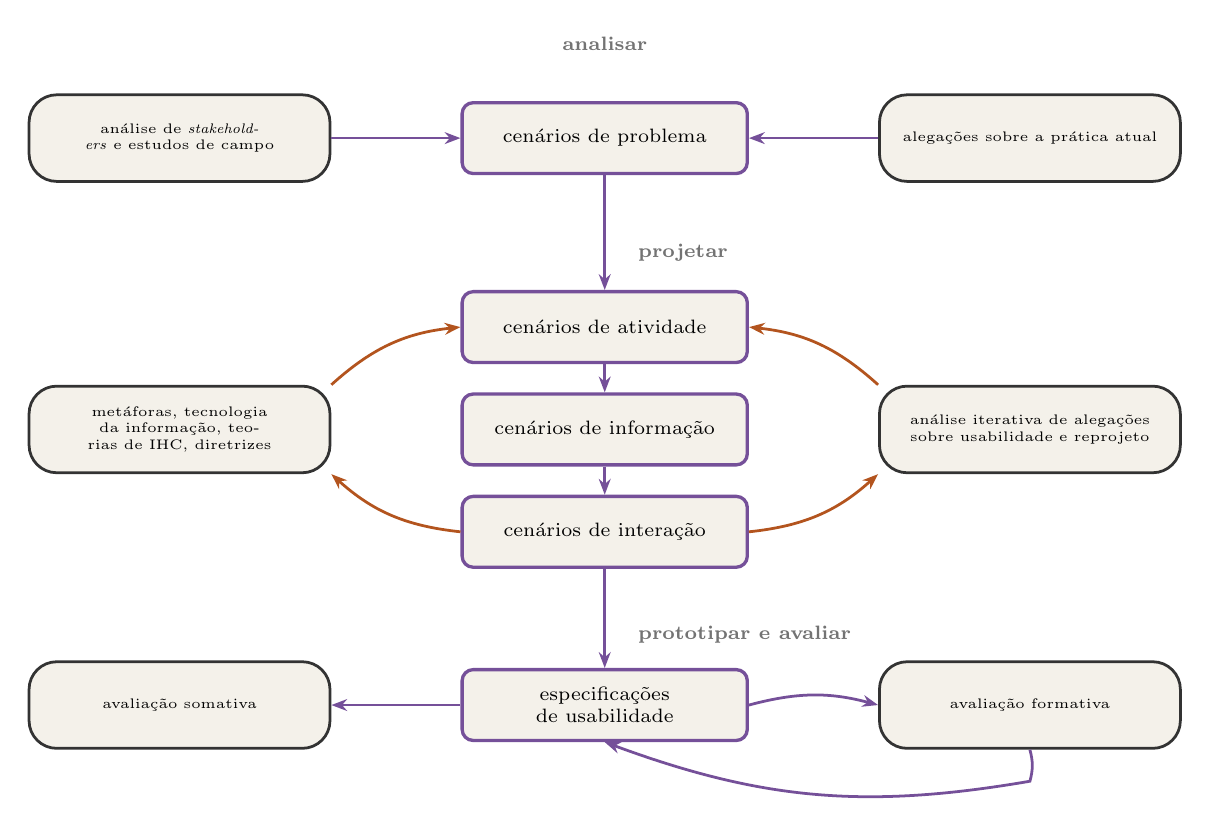
\begin{tikzpicture}[x=1cm,y=1cm,
   pill/.style={dbox, rounded corners=10pt, text width=3.4cm, minimum height=1.1cm, font=\tiny},
   main/.style={dbox, rounded corners=4pt, text width=3.2cm, minimum height=0.9cm, font=\scriptsize, draw=dblue, line width=1.2pt}]

  \node[dlbl, font=\scriptsize\bfseries] at (6.4,6.4) {analisar};
  \node[pill] (s) at (1.0,5.2) {análise de \textit{stakeholders} e estudos de campo};
  \node[main] (cp) at (6.4,5.2) {cenários de problema};
  \node[pill] (al) at (11.8,5.2) {alegações sobre a prática atual};
  \draw[dtrans] (s) -- (cp); \draw[dtrans] (al) -- (cp);

  \node[dlbl, font=\scriptsize\bfseries, anchor=west] at (6.7,3.75) {projetar};
  \node[main] (ca) at (6.4,2.8) {cenários de atividade};
  \node[main] (ci) at (6.4,1.5) {cenários de informação};
  \node[main] (cx) at (6.4,0.2) {cenários de interação};
  \draw[dtrans] (cp) -- (ca); \draw[dtrans] (ca) -- (ci); \draw[dtrans] (ci) -- (cx);
  \node[pill] (m) at (1.0,1.5) {metáforas, tecnologia da informação, teorias de IHC, diretrizes};
  \node[pill] (it) at (11.8,1.5) {análise iterativa de alegações sobre usabilidade e reprojeto};
  \draw[dmeas, bend left=18] (m.north east) to (ca.west);
  \draw[dmeas, bend right=18] (it.north west) to (ca.east);
  \draw[dmeas, bend left=18] (cx.west) to (m.south east);
  \draw[dmeas, bend right=18] (cx.east) to (it.south west);

  \node[dlbl, font=\scriptsize\bfseries, anchor=west] at (6.7,-1.1) {prototipar e avaliar};
  \node[main] (es) at (6.4,-2.0) {especificações de usabilidade};
  \node[pill] (so) at (1.0,-2.0) {avaliação somativa};
  \node[pill] (fo) at (11.8,-2.0) {avaliação formativa};
  \draw[dtrans] (cx) -- (es); \draw[dtrans] (es) -- (so); \draw[dtrans, bend left=15] (es.east) to (fo.west); \draw[dtrans, bend left=15] (fo.south) to ++(0,-0.4) to (es.south);

\end{tikzpicture}
\end{document}
